\documentclass{article}
\usepackage{amsfonts, amsmath, amssymb, amsthm} % Math notations imported
\usepackage{enumitem}
\usepackage{graphicx}
\usepackage{setspace}
\usepackage{indentfirst}
\usepackage[margin=1in]{geometry}
\graphicspath{{./images/}} % Path to images



% \begin{figure}[htb!]
%      \centering
%      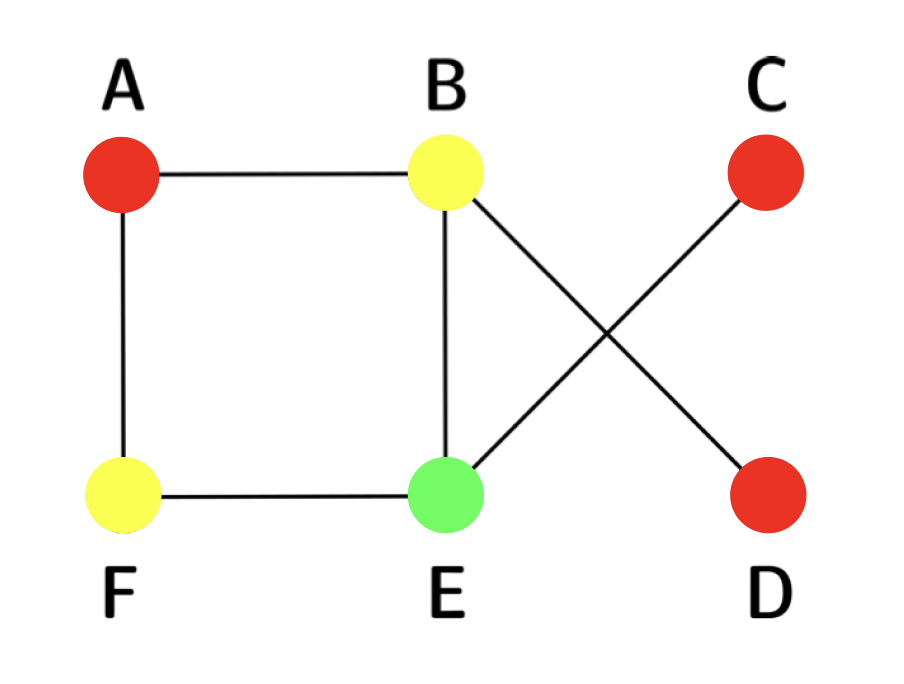
\includegraphics[scale=0.5]{coloring.png}
%      \caption{Coloring of the graph.}
% \end{figure}

% \begin{figure}[htb]
%     \qquad
%     \begin{minipage}{.4\textwidth}
%         \centering
%         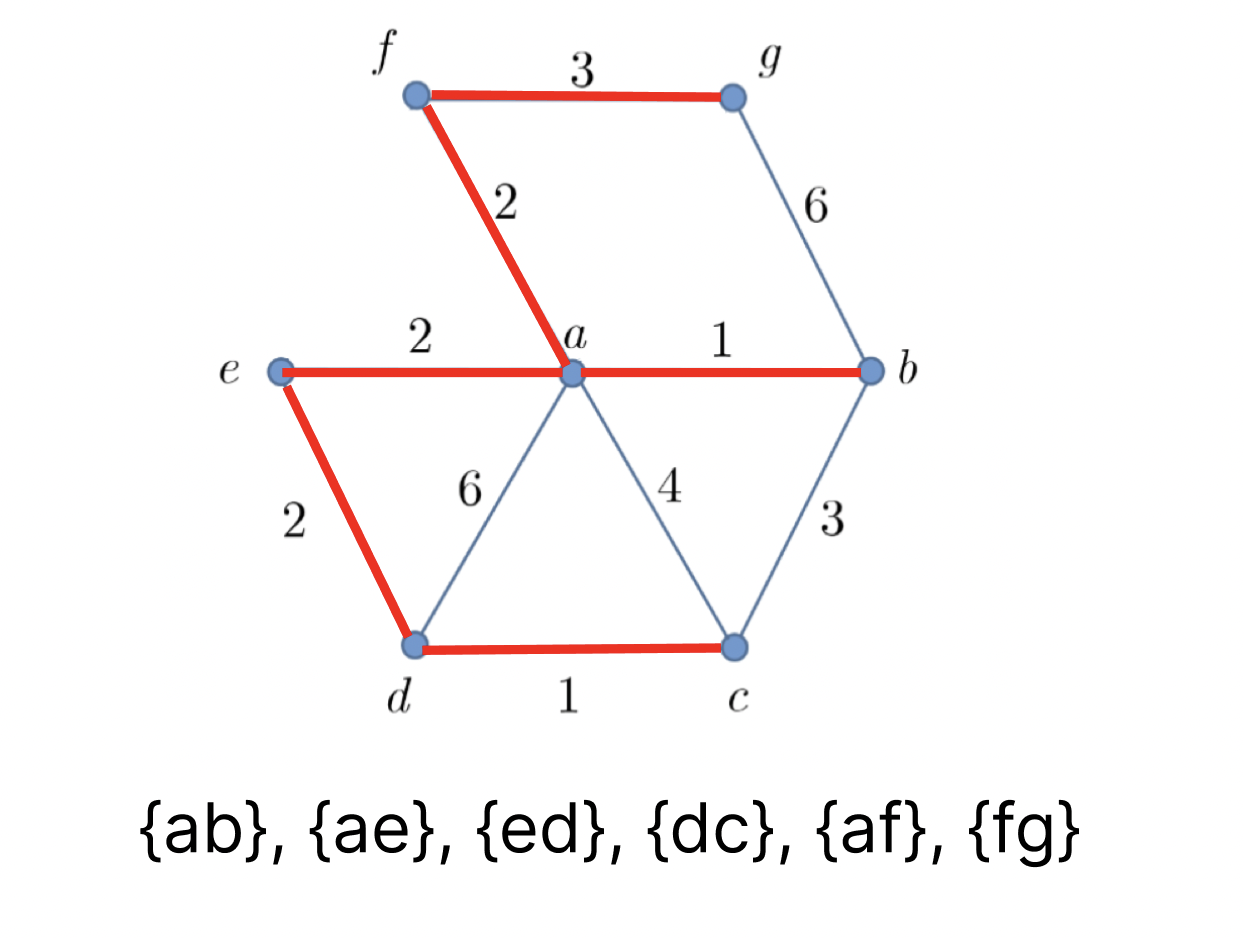
\includegraphics[scale=0.35]{prims.png}
%         \caption{}
%     \end{minipage}    
%     \qquad
%     \begin{minipage}{.4\textwidth}
%         \centering
%         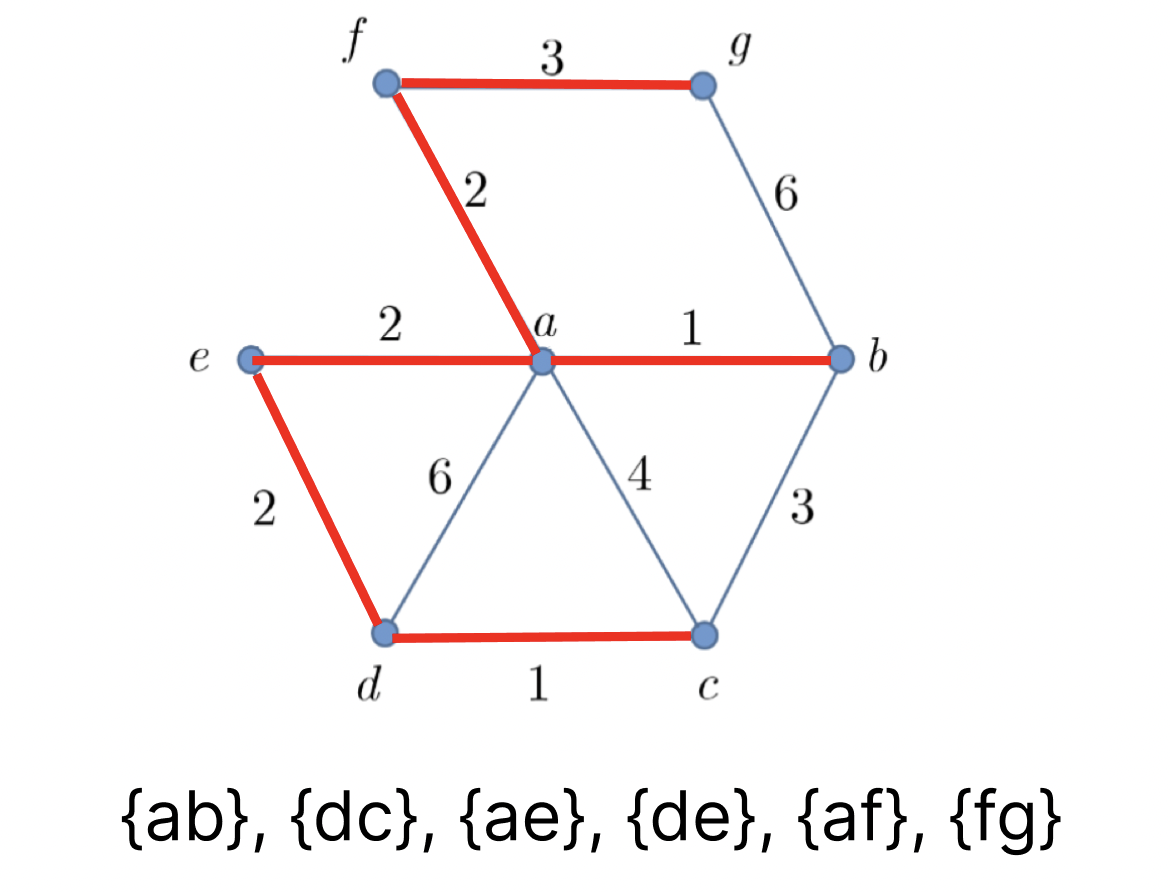
\includegraphics[scale=0.35]{kruskal.png}
%         \caption{}
%     \end{minipage}        
% \end{figure} 

\newtheorem{thm}{Theorem}
\newtheorem{proposition}[thm]{Proposition}
\newtheorem{cor}[thm]{Corollary}

% title information
\title{Math 110 HW5}
\author{Neo Lee}
\date{09/30/2023}



\setstretch{1.15}
% main content
\begin{document} 

% placing title information; comment out if using fancyhdr
\maketitle 

\subsection*{Problem 1.}
Let $V:= \mathbb{C}^3$. Give an example of a map $T\in {\cal L}(V,V)$ such that 
$V=\mathrm{null} T\oplus \mathrm{range} T$, with both $\mathrm{null} T$ and $\mathrm{range} T$ 
non-zero, or prove that none such exists.

\begin{proof}[Solution]
    Let $T:(x,y,z)\mapsto(x,0,0)$ for $x,y,z\in\mathbb{C}$. Then the range of $T$ is 
    $\{(x,0,0):x\in\mathbb{C}\}$, and the null space of $T$ is $\{(0,y,z):y,z\in\mathbb{C}\}$.
    It is obvious that $\mathrm{null}T + \mathrm{range}T = V$ because every $v\in V$ can be written 
    as a sum of a vector in the null space and a vector in the range. 
    Also, $\mathrm{null}T\cap\mathrm{range}T = \{(0,0,0)\}$. Therefore, it is also a direct sum.
\end{proof}

\newpage
\subsection*{Problem 2.}
Given an example of a map $T\in {\mathcal{L}}(\mathbb{R}^6,\mathbb{R}^2)$ such that
$$ \mathrm{null} T =\{(x_1,x_2,x_3,x_4,x_5,x_6) : x_1=-x_2, \;\; x_3+x_5 =0, \;\; x_1-x_4-x_5=0\}$$
or prove that none such exists.
\begin{proof}[Solution]
    We claim that such a map does not exist. Assume for the sake of contradiction that such a map
    $T$ exists.

    Let's rewrite the null space of $T$ as
    $$ \mathrm{null} T =\{(x_1,-x_1,-x_5,x_1-x_5,x_5,x_6) : x_1, x_5, x_6\in\mathbb{R}\}.$$
    In other words, null$T$ is the span of the vectors $(1,-1,0,1,0,0)$, $(0,0,-1,-1,1,0)$, and 
    $(0,0,0,0,0,1)$. We can check whether these three vectors are linearly independent to find the 
    exact dimension of null$T$ but it is unnecessary for this problem. 
    
    Since null$T$ is defined by a span of three vectors, the maximum dimension of null$T$ is 3. 
    Then, by the rank-nullity theorem, the dimension of the range of $T$ is at least $6-3=3$. 
    However, the range of $T$ is a subspace of $\mathbb{R}^2$, so the dimension of the range of $T$ 
    is at most 2. This is a contradiction. Therefore, such a map $T$ does not exist.
\end{proof}


\newpage
\subsection*{Problem 3.}
Suppose $T: {\mathcal{P} }_3(\mathbb{R}) \to {\mathcal{P} }_2(\mathbb{R})$ is defined by the 
formula $(Tf)(x)=4xf''(x)-f'(x)$. Check that
$T\in {\mathcal{L} } ({\mathcal{P} }_3(\mathbb{R}), {\mathcal{P} }_2(\mathbb{R}))$ and find a 
basis for the null space and a basis for the range of $T$.
\begin{proof}[Solution]
    To check whether T is a linear map, we need to check whether $T$ follows additivity and
    homogeneity. 
    
    \textbf{Additivity:} Let $f,g\in{\mathcal{P} }_3(\mathbb{R})$. Then
    \begin{align*}
        T(f+g)(x) &= 4x(f+g)''(x) - (f+g)'(x) \\
        &= 4x(f''+g'')(x) - (f'+g')(x) \\
        &= 4xf''(x) + 4xg''(x) - f'(x) - g'(x) \\
        &= T(f)(x) + T(g)(x).
    \end{align*}

    \textbf{Homogeneity:} Let $f\in{\mathcal{P} }_3(\mathbb{R})$ and $c\in\mathbb{R}$. Then
    \begin{align*}
        T(cf)(x) &= 4x(cf)''(x) - (cf)'(x) \\
        &= 4x(c(f'')'(x)) - cf'(x) \\
        &= 4cx(f'')'(x) - cf'(x) \\
        &= c(4xf''(x) - f'(x)) \\
        &= cT(f)(x).
    \end{align*}

    \textbf{Range:} Let $v\in\mathcal{P}_3(\mathbb{R})$, which can be written as
    $ax^3 + bx^2 + cx + d$ for $a,b,c,d\in\mathbb{R}$. Then, after applying $T$ to $v$, we get 
    \begin{align*}
        T(v)(x) &= 4xv''(x) - v'(x) \\
        &= 4x(6ax + 2b) - (3ax^2 + 2bx + c) \\
        &= 24ax^2 + 8bx - 3ax^2 - 2bx - c \\
        &= 21ax^2 + 6bx - c,
    \end{align*}
    which is a linear combination of $x^2$, $x$, and $1$. Therefore, the range of $T$ is 
    $\mathrm{span}\{x^2, x, 1\}$.

    \textbf{Null Space:} Let $v\in\mathcal{P}_3(\mathbb{R})$, $ax^3 + bx^2 + cx + d$, such that 
    $T(v)(x) = 0$. From what we have derived for range$T$, it means for all $x$
    \begin{align*}
        21ax^2 + 6bx - c &= 0.
    \end{align*}
    This is only possible when $21a = 6b = c = 0$ because $x^2, x, 1$ are linearly independent, in 
    fact basis. Therefore, all vectors in the null space of $T$ are of the form $ax^3 + bx^2 + cx + d$
    where $a=b=c=0$. In other words, the null space of $T$ is span$\{1\}$, or equivalently 
    $\mathbb{R}$. Hence, the basis is $\{1\}$.
\end{proof}

\newpage
\subsection*{Problem 4.}
Let $T :  f(x)\mapsto (x-1)^2f'''(x)-3(x-1)f''(x)+f'(x)$. Write down its matrix representation:
\begin{description}
\item{(a)} as a map in ${\cal L}({\cal P}_3,{\cal P}_2)$ using the standard monomial bases both for 
the domain and codomain;
\item{(b)} as a map in ${\cal L}({\cal P}_3, {\cal P}_3)$ using the standard monomial basis both 
for the domain and codomain;
\item{(c)} as a map in ${\cal L}({\cal P}_3 , {\cal P}_3)$ using the shifted monomial basis 
$1, x-1, (x-1)^2, (x-1)^3$ for the domain and  for the codomain.
\end{description}
\begin{proof}[Solution]\indent
    \begin{enumerate}[label=(\alph*)]
        \item
        \begin{align*}
            T(x^3) & = (x-1)^2(6) - 3(x-1)(6x) + 3x^2 \\
            & = 6x^2 - 12x + 6 - 18x^2 + 18x + 3x^2 \\
            & = -9x^2 + 6x + 6 \\
            T(x^2) & = -3(x-1)(2) + 2x \\
            & = -6x + 6 + 2x \\
            & = -4x + 6 \\
            T(x) & = 1 \\
            T(1) & = 0.
        \end{align*}
        Hence, the matrix representation is 
        \begin{align*}
            \begin{bmatrix}
                -9 & 0 & 0 & 0 \\
                6 & -4 & 0 & 0 \\
                6 & 6 & 1 & 0
            \end{bmatrix}.
        \end{align*}

        \item 
        The matrix representation is simply prepending an empty row at the top of the matrix from 
        (a):
        \begin{align*}
            \begin{bmatrix}
                0 & 0 & 0 & 0 \\
                -9 & 0 & 0 & 0 \\
                6 & -4 & 0 & 0 \\
                6 & 6 & 1 & 0
            \end{bmatrix}.
        \end{align*}

        \item 
        \begin{align*}
            T\left((x-1)^3\right) & = (x-1)^2(6) - 3(x-1)(6(x-1)) + 3(x-1)^2 \\
            & = 6(x-1)^2 - 18(x-1)^2 + 18(x-1)^2 \\
            & = 6(x-1)^2 \\
            T\left((x-1)^2\right) & = -3(x-1)(2) + 2(x-1) \\
            & = -6(x-1) + 2(x-1) \\
            & = -4(x-1) \\
            T\left((x-1)\right) & = 1 \\
            T\left(1\right) & = 0.
        \end{align*}
        Hence, the matrix representation is
        \begin{align*}
            \begin{bmatrix}
                0 & 0 & 0 & 0 \\
                6 & 0 & 0 & 0 \\
                0 & -4 & 0 & 0 \\
                0 & 0 & 1 & 0
            \end{bmatrix}.
        \end{align*}
    \end{enumerate}

    
\end{proof}

\newpage
\subsection*{Problem 5.}
Suppose $V$ and $W$ are finite-dimensional vector spaces.
Let $v$ be a fixed vector in $V$, and consider
$$ E_v := \{ T\in {\cal L}(V,W): Tv=0 \}.$$
\begin{description}
\item{(a)} Show that $E_v$ is a subspace of ${\cal L}(V,W)$.
\item{(b)} Suppose $v\neq 0$. What is $\dim E_v$?
\end{description}
\begin{proof}[Solution]\indent
    \begin{enumerate}[label=(\alph*)]
        \item 
        Firstly, $E_v$ is obviously a subset of $\mathcal{L}(V,W)$.


        \textbf{Additive identity:} The zero map from $V$ to $W$ is obviously in $E_v$ because it 
        maps every vector, including $v$, to $0$. Hence, the additive identity, which is the zero 
        map, is in $E_v$.

        \textbf{Closed under addition:} Let $T_1, T_2\in E_v$. Then 
        \begin{align}
            (T_1+T_2)v &= T_1v + T_2v \\
            & = 0 + 0 \nonumber \\
            & = 0. \nonumber
        \end{align}
        (1) is possible because $T_1, T_2$ are in $\mathcal{L}(V,W)$. Therefore, $T_1+T_2\in E_v$.

        \textbf{Closed under scalar multiplication:} Let $T\in E_v$ and $c\in\mathbb{R}$. Then
        \begin{align}
            (cT)v &= c(Tv) \\
            & = c0 \nonumber \\
            & = 0. \nonumber
        \end{align}
        (2) is possible because $T$ is in $\mathcal{L}(V,W)$. Therefore, $cT\in E_v$.

        \item
        We can construct a basis of $V$ that includes $v$, denoted as 
        $(v, v_2, \dots, v_n)$. Then consider arbitrary $T\in\mathcal{L}(V,W)$ and $z\in V$, 
        \begin{align*}
            T(z) & = T(c_1v + c_2v_2 + \dots + c_nv_n) \\
            & = c_1T(v) + c_2T(v_2) + \dots + c_nT(v_n) \\
            & = c_2T(v_2) + \dots + c_nT(v_n) \\
            & = T(c_2v_2 + \dots + c_nv_n).
        \end{align*}
        
        We can see that $T$ is completely determined by its action on $v_2, \dots, v_n$. Therefore, 
        we can define a map $\Phi:E_v\to\mathcal{L}(V',W)$, 
        $V'=\mathrm{span}\{v_2,\dots,v_m\}$ by restricting the domain of $T$ to 
        $V'$. This map is well-defined as we saw from the above derivation.
        We will show that $\Phi$ is an isomorphism.

        \textbf{Linearity of $\Phi$:}
        \begin{enumerate}[label=(\roman*)]
            \item 
            Let $T_1, T_2\in\mathcal{L}(V,W)$ and $z\in V'$. Then
            \begin{align*}
                \Phi(T_1+T_2)(z) & = (T_1+T_2)(z) \\
                & = T_1(z) + T_2(z) \\
                & = \Phi(T_1)(z) + \Phi(T_2)(z).
            \end{align*}

            \item 
            Let $T\in\mathcal{L}(V,W)$, $c\in\mathbb{R}$, and $z\in V'$. Then
            \begin{align*}
                \Phi(cT)(z) & = (cT)(z) \\
                & = cT(z) \\
                & = c\Phi(T)(z).
            \end{align*}
        \end{enumerate}

        \textbf{Injectivity of $\Phi$:} Let $\Phi(T)=T'\in\mathcal{L}(V',W)$ be the zero map. Then 
        $T'$ maps every vector of $V'$, including the basis to 0. Then, $T$ must map every $v_i$ for 
        $i\in[2,n]$, also the fixed $v$ obviously, to 0 because $T$ have the same actions as $T'$ on 
        $V'$. 
        Hence, $T$ maps every basis in $V$ to zero, consequently every vectors in $V$ to zero. 
        Therefore, $T$ is the zero map and $\Phi$ is injective.

        \textbf{Surjectivity of $\Phi$:} We know $\Phi$ has to be surjective because of how we 
        defined $\Phi$. Every $T'\in \mathcal{L}(V',W)$ has a corresponding $T\in\mathcal{L}(V,W)$ 
        that perform the same action on $V'$ as $T'$ does. Therefore, $\Phi$ is surjective.

        \textbf{$\Phi$ is isomorphism:} We have shown that $\Phi$ is linear, injective, and 
        surjective. Therefore, $\Phi$ is an isomorphism between $E_v$ and $\mathcal{L}(V',W)$. 
        Therefore, $\dim E_v = \dim \mathcal{L}(V',W)=\dim W \times \dim V' = \dim W \times 
        (\dim V - 1)$
        
    \end{enumerate}
\end{proof}

\end{document}